Software synthesis can be seen as embedded in a spectrum of design approaches going from hardware design (and classical \ac{EDA}) through hardware-software co-design up to software synthesis on the other end. 
In software synthesis we strive to derive an efficient execution from a computation expressed in an abstract model to a concrete architecture.
In order to understand software synthesis, thus, we first need to understand the underlying models of computation.
Closely related to these concurrent models of computation are execution traces, which capture a concrete execution for some input.
However, going from such abstract models to a concrete execution also requires an understanding of the target hardware architecture.
The relationship between the two can be captured in a mapping.
This chapter considers all of these aspects with their corresponding models, and the relationship between them.
It is the central piece of background theory required for the methods presented in this thesis.

\subsection{Kahn Process Networks}

The flow we investigate in Part I is based on the \ac{MoC} of \acfp{KPN}.
In this section we introduce this model, or rather, its most common implementation with blocking-read semantics~\cite{kahn_macqueen} .
In Part II, specifically in Chapter~\ref{chap:mocs} we will discuss the original formal semantics~\cite{kahn74} and how they differ to those introduce here.
We also discuss other models of computation and how they relate to each other.

We can think of a \ac{KPN} as a computation distributed among different \emph{processes}\index{KPN ! process} (originally derived from coroutines).
Each of these processes executes sequentially and is Turing complete. However, the processes share no memory, they have memories local only to themselves.
They communicate between each other using \emph{channels}\index{KPN ! channel}, which work as unbounded \acs{FIFO} buffers. 
Processes have sets of outgoing and incoming channels.
As an instruction, any process can write to one of its outgoing channels or read from one of its incoming channels.
They do so in discrete tokens of data.

The original language~\cite{kahn_macqueen} was proposed as an extension of POP-2, which is pretty dated and has fallen out of use today.
Instead of this language, we will consider a more modern incarnation, \ac{CPN}, which extends the C programming language~\cite{cpn}\index{CPN}.
We do so by looking at the example from Listing~\ref{listing:fft_cpn}. 
Processes in \ac{CPN} are instantiated from process templates, similar to classes and objects in object-oriented languages.
The listing shows a very simplified process template for an \acs{FFT} process. 
Lines 2 and 3 declare the incoming and outgoing channels for the process.
In Line 5, the \texttt{cnt} channel is read and its value is stored in the local variable \texttt{loop\_cnt} in Line 6.
Then in Lines 7-10 the process applies an \acs{FFT} to the data in its incoming channel \texttt{src\_data} and outputs it to an outgoing channel, \texttt{freq}. 
Similar to the read operation in Lines 5-6, the values of the input channel data are available in the identifier \texttt{src\_data} in the scope of the \texttt{\_\_PNin}.
In an analogous fashion, the values written to the \texttt{freq} variable in the scope of the \texttt{\_\_PNout} are written to the corresponding output channel.

\begin{listing}
\begin{minted}[linenos]{C}
__PNkpn fft_process
    __PNin(int cnt, short src_data[N])
    __PNout(complex freq[N]){
  int i, loop_cnt;
  __PNin(cnt)
     loop_cnt = cnt;
  for(i = 0; i < cnt; ++i)
    __PNin(src_data) __PNout(freq)
      fft(src_data, freq);
}
\end{minted}
\caption{An \ac{FFT} implemented as a \ac{KPN} process in \ac{CPN}, based on Appendix A.1.3 of \cite{castrillon2014thesis}}
\label{listing:fft_cpn}
\end{listing}


In general, the communication in \acp{KPN} is asynchronous: 
When a process writes to an outgoing channel, the data is buffered in the channel until it is read, and the process continuous to execute.
If a process reads from a channel, it receives the oldest token buffered in the channel.
If there are no tokens, execution blocks until such a token is written to a channel - hence the name, blocking-read semantics.
A channels can be the outgoing channel of at most one process (it should also be so for at least one process, otherwise the channel is useless).
On the other hand, if a channel is an incoming channel to multiple processes, all tokens are copied for each of those processes.
Hence, all processes will see the exact same incoming stream of tokens from a shared channel, instead of splitting them up.

Let us consider the \acs{FFT} process from Listing~\ref{listing:fft_cpn} and combine it with other processes into a full application.
Listing~\ref{listing:audio_filter} describes a simplified algorithm for a low-pass filter on a stereo sound file, using this \acs{FFT} process.
We also omit the templates and channel declarations in this simplified listing.
The \texttt{src} process reads the stereo file, splits it into two channels and sends the sound in blocks of a determined length as tokens.
These files are then transformed from the time domain to the frequency domain using a \acf{FFT}, filtered and transformed back to the time domain.
A sink channel gathers the filtered blocks from both channels, left and right, and combines them again into a stereo sound file that it can store.

\begin{listing}
\begin{minted}{C}
__PNprocess src = src_process
  __PNout(cnt, src_l_out, src_r_out);
__PNprocess fft_l = fft_process
  __PNin(count, src_l_out) __PNout(fft_l_out);
__PNprocess fft_r = fft_process
  __PNin(count, src_r_out) __PNout(fft_r_out);
__PNprocess filter_l = filter_process
  __PNin(count, fft_l_out) __PNout(filter_l_out);
__PNprocess filter_r = filter_process
  __PNin(count, fft_r_out) __PNout(filter_r_out);
__PNprocess ifft_l = ifft_process
  __PNin(count, filter_l_out) __PNout(ifft_l_out);
__PNprocess ifft_r = ifft_process
  __PNin(count, filter_r_out) __PNout(ifft_r_out);
__PNprocess sink = sink_process
  __PNin(count, ifft_l_out, ifft_r_out);
\end{minted}
\caption{An audio filter \ac{KPN} application in \ac{CPN}, based on Figure 7a in \cite{cpn}}
\label{listing:audio_filter}
\end{listing}

The data flow in the example of Listing~\ref{listing:audio_filter} is very structured: it goes from the source, split over both channels, through the filter, back to the sink.
This structure can easily be visualized in a graph, like in Figure~\ref{fig:audio_filter_graph}.
More generally, we can think of any \ac{KPN} application as a directed graph $K = (V_K,E_K)$, where the nodes $V_K$ represent the processes, and the edges $E_K$, the channels.
This works even when a channel is an incoming channel for multiple processes.
In that case, we can split it into multiple edges from the process it is going from, to each of the target channels.
We can do so without loss of generality since these are the semantics of such channels. 
We call this graph the \emph{\ac{KPN} graph}\index{KPN ! graph}.

\begin{figure}[h]
	\centering
\resizebox{0.9\textwidth}{!}{
\begin{tikzpicture}
   \node[draw, ellipse,minimum width = 1.1cm, minimum height=0.9cm] (src) {src};
\node[draw, ellipse,minimum width = 1.1cm, minimum height=0.9cm, below right = 1cm of src] (fft_l) {\texttt{fft\_l}};
\node[draw, ellipse,minimum width = 1.1cm, minimum height=0.9cm, above right = 1cm of src] (fft_r) {\texttt{fft\_r}};
\node[draw, ellipse,minimum width = 1.1cm, minimum height=0.9cm, right = 1 cm of fft_l] (filter_l) {\texttt{filter\_l}};
\node[draw, ellipse,minimum width = 1.1cm, minimum height=0.9cm, right = 1 cm of fft_r] (filter_r) {\texttt{filter\_r}};
\node[draw, ellipse,minimum width = 1.1cm, minimum height=0.9cm, right = 1 cm of filter_l] (ifft_l) {\texttt{ifft\_l}};
\node[draw, ellipse,minimum width = 1.1cm, minimum height=0.9cm, right = 1 cm of filter_r] (ifft_r) {\texttt{ifft\_r}};
\node[draw, ellipse,minimum width = 1.1cm, minimum height=0.9cm, below right = 1cm of ifft_r] (sink) {\texttt{sink}};

\draw[-latex] (src) -- (fft_l);
\draw[-latex] (src) -- (fft_r);
\draw[-latex] (fft_l) -- (filter_l);
\draw[-latex] (fft_r) -- (filter_r);
\draw[-latex] (filter_l) -- (ifft_l);
\draw[-latex] (filter_r) -- (ifft_r);
\draw[-latex] (ifft_l) -- (sink);
\draw[-latex] (ifft_r) -- (sink);
 \end{tikzpicture}
}
   \caption{The audio filter application as a \ac{KPN} graph}
	\label{fig:audio_filter_graph}
\end{figure}

\subsection{Execution Traces}

Kahn Process Networks have a more abstract definition with mathematical semantics~\cite{kahn74}, in the sense of Scott~\cite{scott1970}.
These abstract away the concrete implementation of individual steps in a computation.
Even so, the execution of a computation can be thought of as a series of steps or partial computations that eventually yield the final result.
These series, which is commonly referred to as execution trace, can be captured as a sequence of steps, e.g. as the element of a Scott Domain\footnote{this will all be discussed more in-depth in Chapter~\ref{chap:mocs}}. 
Abstract computations, modeled as Scott-continuous functions, can can make computations of arbitrary length.
For an alphabet $D$, this is modeled by (countably) infinite sequences in $D^\omega \setminus D^* = \{ (a_n)_{n \in \mathbb{N}} \mid a_n \in D \text {for all} n \in \mathbb{N} \}$.
A concrete execution, on the other hand, always has a finite length.
It always resides in $D^*$, the Kleene colsure of $D$.
For a (Scott-continuous) function, this sequence can be modeled as a finite string in the computation domain.

In a concurrent execution, multiple entities concurrently execute steps.
As modeled by Kahn, these entities all implement individual (Scott-continuous) functions.
As such, there is not a unique series of steps that can be said to be the execution trace of the computation.
To see this, consider the example depicted in Figure~\ref{fig:audio_fiter_traces}:
\todo{finish, discuss example. Is this trace the right way of doing it? (should be reads and writes to channels for the individual histories)}

\begin{figure}[h]
	\centering
   \resizebox{0.7\textwidth}{!}{\small
\tikzstyle{terminal}=[rectangle,draw,fill=black!10,minimum height=0.5cm]
\tikzstyle{edge}=[->,align=center]
\newcommand{\mktwithoutedge}[1]{
  \node[terminal,right=of tnode] (tnode) {#1};
}
\newcommand{\mkt}[1]{
  \mktwithoutedge{#1}
  \draw[edge] (tnode.east) -- ($(tnode.east)+(0.13,0)$);
}
\newcommand{\connect}[2]{
  \draw[edge] (#1) -- (#2);
}
\begin{tikzpicture}
  % Tokens
  \begin{scope}[node distance=0.5cm and 0.13cm]
    \begin{scope}[node distance=0.4]
      \node[] (a1) {};
      \node[below=of a1] (a2) {};
      \node[below=of a2] (a3) {};
      \node[below=of a3] (a4) {};
      \node[below=of a4] (a5) {};
    \end{scope}

    \begin{scope}[opacity=1]
    \node[left=of a1] (tnode) {};
      \mkt{src}
      \mkt{fft\_l}
      \mkt{fft\_r}
      \mkt{filter\_l}
      \mkt{filter\_r}
      \mkt{ifft\_l}
      \mkt{ifft\_r}
      \mktwithoutedge{sink}
    \end{scope}

    \begin{scope}[opacity=1]
      \node[left=of a2] (tnode) {};
      \mkt{src}
      \mkt{fft\_l}
      \mkt{filter\_l}
      \mkt{ifft\_l}
      \mkt{fft\_r}
      \mkt{filter\_r}
      \mkt{ifft\_r}
      \mktwithoutedge{sink}
    \end{scope}

    \begin{scope}[opacity=1]
      \node[left=of a3] (tnode) {};
      \mkt{src}
      \mkt{fft\_l}
      \mkt{filter\_l}
      \mkt{fft\_r}
      \mkt{ifft\_l}
      \mkt{filter\_r}
      \mkt{ifft\_r}
      \mktwithoutedge{sink}
    \end{scope}

    \begin{scope}[opacity=1]
      \node[left=of a4] (tnode) {};
      \mkt{src}
      \mkt{fft\_r}
      \mkt{filter\_r}
      \mkt{fft\_l}
      \mkt{filter\_l}
      \mkt{ifft\_l}
      \mkt{ifft\_r}
      \mktwithoutedge{sink}
    \end{scope}

    \begin{scope}[opacity=1]
      \node[left=of a5] (tnode) {};
      \mkt{src}
      \mkt{fft\_l}
      \mkt{filter\_l}
      \mkt{fft\_r}
      \mkt{filter\_r}
      \mkt{ifft\_l}
      \mkt{ifft\_r}
      \mktwithoutedge{sink}
    \end{scope}

  \end{scope}

\end{tikzpicture}
}
   \caption{Different possible executions of the audio \ac{KPN}.}
	\label{fig:audio_filter_traces}
\end{figure}


In the distributed case thus, the execution traces are in fact equivalence classes of strings.
We define this more formally, following~\cite{mazurkiewicz1995introduction}, the first chapter of~\cite{diekert1995book}.
Let $D$ be a finite set, like an alphabet $\Sigma$ or data type $D = \Cup_{i \in \mathcal{I}} D_i$ be a data type for a \ac{KPN}.
Let $\Delta$ be a symmetric, reflexive relation on $D$, which we call a dependency\index{dependency}.
This means that if $(a,b) \in \Delta$, we have $(b,a) \in \Delta$ and also $(a,a) \in Delta$ for all $a \in D$. 
With $\Delta$ we define an additional relation in $D$, namely $I := (D \times D) \setminus \Delta$.
We call $I$ the induced independency\index{independency}. 
We define an equivalence relation $\sim_I$ on the monoid $D^*$ (with respect to concatenation) as follows:
We require for $a,b \in I$ then $ab \sim_I ba$. The relation $\sim_I$ is defined as the least congruence that satisfies this requirement.
Note that a congruence is an equivalence relation that respects the algebraic structure, in this case the monoid structure of the concatenation operation.
We call the equivalence classes of $D^*/{\sim_I}$ traces. 
By definition, the concatenation operation on $D^*$ factors over the equivalence relation $\sim_I$,
and thus $D^*/{\sim_I}$ defines a monoid (with identity element $[\epsilon]_{\sim_i}$, where $\epsilon \in D^*$ is the empty string).
We call this the Trace Monoid\index{trace monoid}, $T(D)$.
We care about the algebraic structure of a monoid since it is central to the definition of Scott-continuity.

\begin{ex}
  Todo (based on example above)
\end{ex}

There are two additional equivalent definitions of this monoid as histories and dependence graphs.
We present histories here, as they are easier for the intuition.
Instead of a single alphabet (or set of types) $D$, we have a finite set of alphabets $D := (D_i), i \in \mathcal{I}$, where $\mathcal{I}$ is a finite index set.
We can think of the indices as corresponding to the processes or actors in the system, and the alphabets $D_i$ to the alphabets of these individual entities.
If we think of the individual entities as computing some (Scott-continuous) function, their execution trace will be a unique string $a_i \in D_i^*$ (recall that concrete executions are finite).
Since, in general, these entities do not compute independently, they have common synchronization points.
These synchronization points are abstractly modeled in the computation alphabet by mutual elements in $D_i \cap D_j$ for two entities $i,j \in \mathcal{I}$.
We can define a monoid, the product monoid~\index{product monoid} $P(D)$, by component-wise concatenation of the strings: $(a_i)_i (b_i)_i = (a_ib_i)_i$ for all $i \in \mathcal{I}$.
However, not every such a string product can be the history of a system.
The synchronization points of different subsystems should be consistent with each other. Consider the following example:
\begin{ex}
  \label{ex:inconsistency_history}
TODO: slight variation that shows an element of $P(D) \setminus H(D)$
\end{ex}
To avoid this, we want to ensure histories are consistent. For this, we define elementary histories~\index{elementary history} as follows:
For any $a in \Cup_{i \in \mathbb{I}} D_i$, the elementary history of $a$ is the tuple $(a_i)_{i \in \mathbb{I}}$, with $a_i = \left\{ \begin{array}{ll} a, & \text{ if } a \in D_i, \\ \epsilon, & \text{ otherwise. }\end{array}\right.$
Again, $\epsilon$ represents the empty string.
The monoid generated by all elementary histories for elements in $\Cup_{i \in \mathbb{I}} D_i$ is called the history monoid $H(D)$, and is a submonoid of $P(D)$.
If we examine the definition, it is not difficult to convince ourselves that these are precisely the histories which avoid inconsistencies like those of Example~\ref{ex:inconsistency_history}.

\begin{ex}
  Todo (based on example above)
\end{ex}

We can go from a trace to a history by the morphism $\pi: T(\Cup_{i \in \mathcal{I}}) \rightarrow H(D), a \mapsto (\pi_i(a))_i, i \in \mathcal{I}$, where $\pi_i$ is the projection $\Cup_{i \in \mathcal{I}}D_i \rightarrow D_i$.
Here, for the trace monoid $T(D)$ we define the dependencies to be $\Cup_{i \in \mathcal{I}}D_i \times D_i$. 
This is not just a morphism, but in fact an isomorphism: See Theorem 1.5.4 of~\cite{mazurkiewicz1995introduction}.
Thus, the two concepts are equivalent.
For the rest of this thesis we will use the terms traces and histories interchangeably.


Traces, and equivalently histories, can be used to describe the concrete computations in concurrent systems like those described by a \ac{KPN}.
They are also well-suited (and well-suited) to model these systems in the context of process calculi, like \ac{CSP}.
However, an important observation is the converse: a concrete execution of a \ac{KPN} is determined uniquely by its history.
Moreover, any concrete implementation of the \ac{KPN} realizing the same execution will have the same history: the history is an invariant of the abstract execution model.
It captures the concurrent essence of the concrete computation.

\subsection{Architecture Models}
Hardware architectures are in significant contrast to applications from the point of view of modeling.
Abstraction boundaries are more clearly defined in the hardware world: semiconductor components like transistors are organized into digital switches, which are used to form logic gates (like a NAND gate) in logic diagrams for components, like an \ac{ALU}.
These components are combined into digital machines in a microarchitecture to expose a well-defined \acf{ISA} in a \ac{PE}~\cite{lee2017plato}.
\acp{PE} can then be connected via on-chip interconnects to on-chip memory and other controllers to make an \ac{MPSoC}.
The boundaries between these levels of abstraction or \emph{platforms}, as A. Sangiovanni-Vincentelli calls them~\cite{sangiovanni2007quo}, are clear.
Designers at each level expose a small amount of complexity through these established abstractions, in what is commonly referred to an hourglass design~\cite{10.1145/3274770}.

\begin{figure}[h]
	\centering
\resizebox{0.8\textwidth}{!}{
   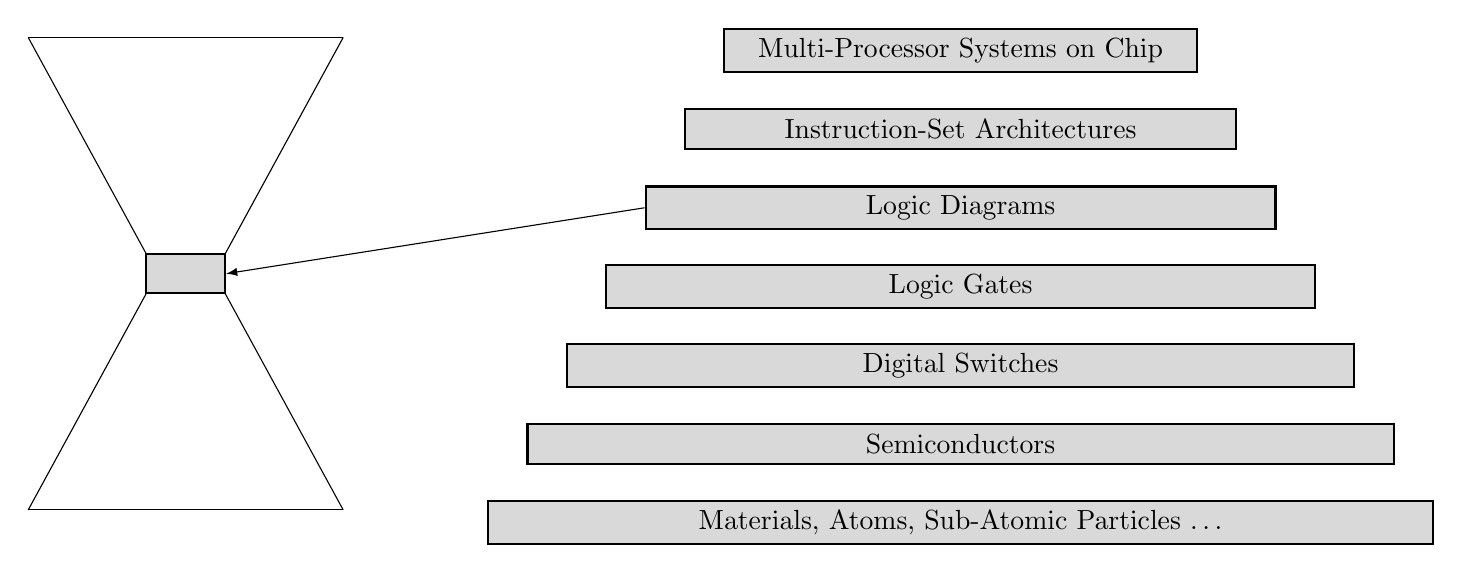
\begin{tikzpicture}
     %layers:
\begin{scope}[scale=1]
  \draw (2.5,0.25) -- (4,3);
\draw (1.5,0.25) -- (0,3);
\draw (1.5,0.25) -- (2.5,0.25);
\draw (4,3) -- (0,3);
\node (interface) at (2,0) [draw,thick,minimum width=1cm,minimum height=0.5cm, fill=gray!30] {};
\draw (2.5,-0.25) -- (4,-3);
\draw (1.5,-0.25) -- (0,-3);
\draw (1.5,-0.25) -- (2.5,-0.25);
\draw (4,-3) -- (0,-3);

\end{scope}

\begin{scope}[xshift = 280,yshift=-90]
\node (physics) at (2,0) [draw,thick,minimum width=12cm,align=center,minimum height=0.5cm, fill=gray!30] {Materials, Atoms, Sub-Atomic Particles $\ldots$};
\node (semiconductors) [draw,above of=physics,thick,minimum width=11cm,align=center,minimum height=0.5cm, fill=gray!30] {Semiconductors};
\node (digital) [draw,above of=semiconductors, thick,minimum width=10cm,align=center,minimum height=0.5cm, fill=gray!30] {Digital Switches};
\node (logic) [draw,above of=digital,thick,minimum width=9cm,align=center,minimum height=0.5cm, fill=gray!30] {Logic Gates};
\node (diagrams) [draw,above of=logic,thick,minimum width=8cm,align=center,minimum height=0.5cm, fill=gray!30] {Logic Diagrams};
\node (isa) [draw,above of=diagrams,thick,minimum width=7cm,align=center,minimum height=0.5cm, fill=gray!30] {Instruction-Set Architectures};
\node (mpsoc) [draw,above of=isa,thick,minimum width=6cm,align=center,minimum height=0.5cm, fill=gray!30] {Multi-Processor Systems on Chip};
\end{scope}

\draw  [-latex] (diagrams.west) -- (interface.east);
   \end{tikzpicture}
 }
   \caption{Different levels of abstraction in architectures}
   \label{fig:architecture_abstractions}
\end{figure}

Figure~\ref{fig:architecture_abstractions} summarizes different models used at different levels in achitecture.
The layer between hardware and software is, in a sense, also just such a layer of abstraction.
Since these layers are very clear in the hardware world, so are the corresponding models at those levels of abstraction.
If we want to reason about the execution of complex applications on \acp{MPSoC}, we certainly should not focus on modeling individual logic gates in the architecture.
The challenge is to model architectures at the right level of abstraction.

In the modeling of the computation in applications, we care about the semantics of the model.
It should be expressive enough to capture the application while being rigid enough to allow a compiler and system to reason about its execution and optimize it as much as possible.
Hardware, on the other hand, is fixed: in software synthesis (and in this thesis) we're not concerned with hardware design.
As such, we take a more scientific role to modeling hardware, as opposed to the engineering role we take for applications: We fit the model to the hardware, not the hardware to the model (cf.~\cite{lee2017plato}).

Architectures models for software synthesis have two main requirements: specification and simulation.
In order to derive an efficient implementation of an application to an architecture, the model of that architecture needs to at least include the possible decisions required for that software implementation.
Different \acp{PE} and their types in the architecture, scratchpad memories or \ac{DMA} controllers, when present, are certainly necessary parts of the models.
If actual physical memory addresses or concrete instructions in the \ac{ISA} should also be included depends on the flow: an end-to-end compiler that produces binaries might benefit from modeling these,
whereas a higher-level, source-to-source compiler might do without them if it only makes abstract decisions about resource allocation and leaves code generation to a separate compiler.


Similarly, in many cases a simulation is part of the software synthesis flow.
In this case, a model of the architecture needs to allow such a simulation.
Obviously, a simple analytic model requires a different level of abstraction for the architecture model than a cycle-accurate simulator.
A very concrete way of considering this is the Y-chart approach proposed in~\cite{kienhuis2001methodology}, as depicted in Figure~\ref{fig:y-charts}, which is based on Figure~6 from~\cite{kienhuis2001methodology}. 

\begin{figure}[h]
	\centering
\resizebox{0.8\textwidth}{!}{
   \begin{tikzpicture}
     
%https://tex.stackexchange.com/questions/343354/tikz-rectangle-with-diagonal-fill-two-colors
\tikzset{
diagonal fill/.style 2 args={fill=#2, path picture={
\fill[#1, sharp corners] (path picture bounding box.south west) -|
                         (path picture bounding box.north east) -- cycle;}},
reversed diagonal fill/.style 2 args={fill=#2, path picture={
\fill[#1, sharp corners] (path picture bounding box.north west) |- 
                         (path picture bounding box.south east) -- cycle;}}
}
\tikzstyle{block} = [rectangle, draw, fill=blue!20, 
    text width=7em, text centered, rounded corners, minimum height=4em]
\tikzstyle{moa} = [rectangle, draw, fill=green!20, 
    text width=7em, text centered, rounded corners, minimum height=4em]
\tikzstyle{both} = [rectangle, draw,diagonal fill={blue!20}{green!20}, 
    text width=7em, text centered, rounded corners, minimum height=4em]

\node[block] (mapping1) {Mapping};
\node[both, above left = of mapping1] (estimation-models) {Estimation \\ Models};
\node[block, above right = of mapping1] (apps1) {Applications};
\node[moa, below = of mapping1] (high-level) {High-level \\ Model \\ (e.g. Matlab/ \\ Mathematica)};
\node[block, below = of high-level] (numbers1) {Performance \\ Numbers};
\draw[-latex,gray] (estimation-models) -- (mapping1);
\draw[-latex,gray] (estimation-models) -- (high-level);
\draw[-latex,gray] (apps1) -- (mapping1);
\draw[-latex,gray] (mapping1) -- (high-level);
\draw[-latex,gray] (high-level) -- (numbers1);


 \node[block, right = 8cm of high-level] (mapping2) {Mapping};
\node[both, above left = of mapping2] (accurate-models) {Accurate \\ Models};
\node[block, above right = of mapping2] (apps2) {Applications};
\node[moa, below = of mapping2] (low-level) {Low-level \\ Simulator \\ (e.g. VHDL/ \\ Cycle-Accurate)};
\node[block, below = of low-level] (numbers2) {Performance \\ Numbers};
\draw[-latex,gray] (accurate-models) -- (mapping2);
\draw[-latex,gray] (accurate-models) -- (low-level);
\draw[-latex,gray] (apps2) -- (mapping2);
\draw[-latex,gray] (mapping2) -- (low-level);
\draw[-latex,gray] (low-level) -- (numbers2);

\draw[-latex,very thick,black] (mapping1) -- (mapping2) node[midway, below ,align=center] {\\ \\ (moving down in the \\ Abstraction Pyramid)};

    \matrix [draw=black,fill=gray!10,above=7em of apps2.north east, anchor=north east] {
      \node[moa, rounded corners=0, text width=1em, minimum height=1em] {}; & \node[] {architecture model}; \\
      \node[block, rounded corners=0, text width=1em, minimum height=1em] {}; & \node[] {other models};\\
      };
   \end{tikzpicture}
 }
   \caption{Multiple Levels of Abstraction in the Y-Chart Approach (Adapted from Figure~6 in ~\cite{kienhuis2001methodology}).}
   \label{fig:y_chart_abstractions}
\end{figure}

The Y-charts approach is closer to a co-design methodology: architectures are part of the design space, albeit only as parametrized families.
As such, they model an architecture as an abstract set of parameters (e.g. number of cores of specified core types) for specification (mapping), with an ad-hoc model for simulation (in matlab/mathematica) or well-defined models from a lower level of abstraction (cycle-accurate models or VHDL).
Thus, the approach described in Figure~\ref{fig:architecture_abstractions} shows well how different models of architectures at different levels of abstraction can co-exist and be used.
While accurate simulation is pivotal for effective software synthesis, simulation methods and accuracy are beyond the scope of this thesis.
We will thus focus only on models of architecture for the sake of \ac{DSE} and the specification of decisions (concretely, here, mappings).

The general situation described in the Y-charts approach is very common in practice: A parametrized family of hardware architectures is assumed as part of the flow, and architectures are described in terms of this family.
With newer developments in hardware, like the proliferation of \ac{NoC}-based architectures, many modern approaches apply the same principle to these modern architectures.
For example, the models used by~\cite{weichslgartner2014daarm,singh2010communication,richthammer2018search} all assume a regular mesh ($N \times M$)\ac{NoC}-based topology and parametrize the architecture by the size of the mesh, $N,M$ as well as the core types and communication and memory parameters like worst-case latency values.
TODO: multi-level (pimentel)

In the DOL approach~\cite{thiele2007DOL}, architectures are modeled in an XML specification that implicitly models the architectures as graphs with specific annotations e.g. for memory sizes or resource sharing methods like \ac{FIFO}. 
While this is an ad-hoc model, its graph-based nature is general enough to describe arbitrary architectures.
This is common of the most general models at this level of abstraction: they are graph-based models.
In Sesame, architectures are modeled with bi-partite graphs~\cite{erbas2006multiobjective} with cores and memories.
This is bi-partite structure is actually similar to the constraint graphs defined in~\cite{weichslgartner2014daarm,richthammer2018search}, which basically describe the subset of the architecture used by a mapping. 
In MAPS~\cite{maps}, on the other hand, for the purposes of mapping, architectures are described by labeled graphs where only the cores are nodes and the edges represent communication.
There are subtle differences between all these models, which makes comparing approaches difficult~\cite{goens_mcsoc16}.

In practice, however, the different graph-based architecture models are mostly equivalent.
For this thesis we use a model based on the the MAPS model for defining \emph{architecture graphs}\index{architecture graph}.
An architecture graph $A = (V_A,E_A,l_A)$ is a labeled directed multigraph where the nodes $V_A$ represent \acp{PE} in the architecture. These \acp{PE} are labeled with core types $l_A(V_A) \subset \{\text{core types}\}$. 
Communication in the achitecture graph is represented by the edges $E_A$. Since $A$ is a multigraph, $E_A$ is a multiset: there can be multiple edges $e_1,\ldots,e_n \in E_A$ between two cores $\text{PE},\text{PE}' \in V_A$.
These edges are different by their label $l_A(e_i), i = 1,\ldots,n$. The labels of edges identify them as \emph{communication primitives}\index{communication primitive}.
Communication primitives are an abstraction that encompasses communication via multiple methods: shared memories, \ac{DMA} or even specialized hardware like hardware \ac{FIFO} buffers.
Communication primitives can also be used to model different software libraries/\acp{API} for communication that can use the same hardware~\cite{odendahl2013split}.

\begin{figure}[h]
	\centering
\resizebox{0.3\textwidth}{!}{
   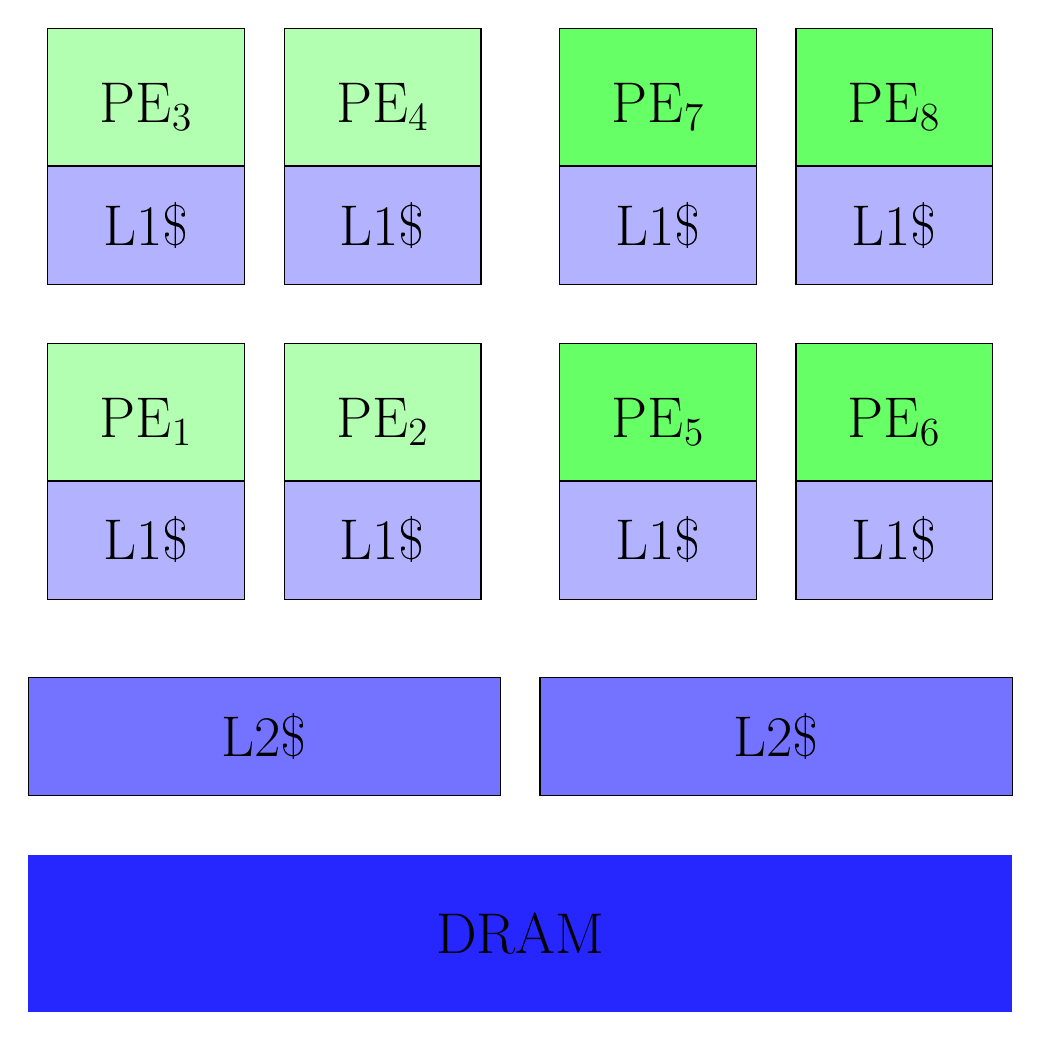
\begin{tikzpicture}
     %little cores
\node (pe1) at ({-1.5},{4}) [draw,minimum width=2.5cm,align=center,minimum height=2cm, fill=green!30] {\huge PE$_1$};
\node (L1-pe1) at (-1.5,2.5) [draw,minimum width=2.5cm,align=center,minimum height=1.5cm, fill=blue!30] {\huge L1\$};
\node (pe2) at (-1.5+3,4) [draw,minimum width=2.5cm,align=center,minimum height=2cm, fill=green!30] {\huge PE$_2$};
\node (L1-pe2) at (-1.5+3,2.5) [draw,minimum width=2.5cm,align=center,minimum height=1.5cm, fill=blue!30] {\huge L1\$};
\node (pe3) at (-1.5,4+4) [draw,minimum width=2.5cm,align=center,minimum height=2cm, fill=green!30] {\huge PE$_3$};
\node (L1-pe3) at (-1.5,2.5+4) [draw,minimum width=2.5cm,align=center,minimum height=1.5cm, fill=blue!30] {\huge L1\$};
\node (pe4) at (-1.5+3,4+4) [draw,minimum width=2.5cm,align=center,minimum height=2cm, fill=green!30] {\huge PE$_4$};
\node (L1-pe4) at (-1.5+3,2.5+4) [draw,minimum width=2.5cm,align=center,minimum height=1.5cm, fill=blue!30] {\huge L1\$};

%big cores
\node (pe5) at ({6.5-1.5},{4}) [draw,minimum width=2.5cm,align=center,minimum height=2cm, fill=green!60] {\huge PE$_5$};
\node (L1-pe5) at (6.5-1.5,2.5) [draw,minimum width=2.5cm,align=center,minimum height=1.5cm, fill=blue!30] {\huge L1\$};
\node (pe6) at (6.5-1.5+3,4) [draw,minimum width=2.5cm,align=center,minimum height=2cm, fill=green!60] {\huge PE$_6$};
\node (L1-pe6) at (6.5-1.5+3,2.5) [draw,minimum width=2.5cm,align=center,minimum height=1.5cm, fill=blue!30] {\huge L1\$};
\node (pe7) at (6.5-1.5,4+4) [draw,minimum width=2.5cm,align=center,minimum height=2cm, fill=green!60] {\huge PE$_7$};
\node (L1-pe7) at (6.5-1.5,2.5+4) [draw,minimum width=2.5cm,align=center,minimum height=1.5cm, fill=blue!30] {\huge L1\$};
\node (pe8) at (6.5-1.5+3,4+4) [draw,minimum width=2.5cm,align=center,minimum height=2cm, fill=green!60] {\huge PE$_8$};
\node (L1-pe8) at (6.5-1.5+3,2.5+4) [draw,minimum width=2.5cm,align=center,minimum height=1.5cm, fill=blue!30] {\huge L1\$};


\node (L2-little) at (0,0) [draw,minimum width=6cm,align=center,minimum height=1.5cm, fill=blue!55] {\huge L2\$};
\node (L2-big) at (6.5,0) [draw,minimum width=6cm,align=center,minimum height=1.5cm, fill=blue!55] {\huge L2\$};
\node (DRAM) at (3.25,-2.5) [minimum width=12.5cm,align=center,minimum height=2cm, fill=blue!85] {\huge DRAM};
   \end{tikzpicture}
 }
   \caption{The Odroid-XU4 Architecture.}
   \label{fig:odroid}
\end{figure}

Consider the architecture depicted in Figure~\ref{fig:odroid},the Exynos Odroid-XU4 with a Samsung Exynos 5422 chip, which has an octocore ARM big.LITTLE (4+4) architecture. 
This architecture has two types of cores, the ARM Cortex A7/A15 , little and  big, respectively. Similarly, there are three types of communication primitives in the architecture:
communication via the L1 and L2 caches, or over the shared DRAM memory.
This architecture can be modeled in an architecture graph by having $8$ nodes, one for each core ($4$ of each of the two core types), and connecting the nodes by with all the primitives that can be used to communicate between them.
Figure~\ref{fig:architecture_graph_odroid} the architecture graph for this example.

\begin{figure}[h]
	\centering
\resizebox{0.8\textwidth}{!}{
   \begin{tikzpicture}
       %cores big
  \node[ellipse,fill=green!30] (pe1) {PE$_1$};
  \node[ellipse,fill=green!30, below right = of pe1] (pe2) {PE$_2$};
  \node[ellipse,fill=green!30, below left = of pe1] (pe3) {PE$_3$};
  \node[ellipse,fill=green!30, below right = of pe3] (pe4) {PE$_4$};

  %cores little
  \node[ellipse,fill=green!60, right = 6 cm of pe1] (pe5) {PE$_5$};
  \node[ellipse,fill=green!60, below right = of pe5] (pe6) {PE$_6$};
  \node[ellipse,fill=green!60, below left = of pe5] (pe7) {PE$_7$};
  \node[ellipse,fill=green!60, below right = of pe7] (pe8) {PE$_8$};
\foreach \c\i in {blue!55/-0.4,blue!85/0.4}{
  %connections big
  \draw[latex-latex,color=\c] ([xshift=\i * 0.1cm,yshift=\i * 0.1cm]pe1.south east) -- ([xshift=\i * 0.1cm,yshift=\i * 0.1cm]pe2.north west);
  \draw[latex-latex,color=\c] ([xshift=\i * -0.1cm,yshift=\i * 0.1cm]pe1.south west) -- ([xshift=\i * -0.1cm,yshift=\i * 0.1cm]pe3.north east);
  \draw[latex-latex,color=\c] ([xshift=\i * 0.1cm,yshift=\i * 0.0cm]pe1.south) -- ([xshift=\i * 0.1cm,yshift=\i * 0.0cm]pe4.north);
  \draw[latex-latex,color=\c] ([xshift=\i * 0.0cm,yshift=\i * 0.1cm]pe2.west) -- ([xshift=\i * 0.0cm,yshift=\i * 0.1cm]pe3.east);
  \draw[latex-latex,color=\c] ([xshift=\i * 0.1cm,yshift=\i * -0.1cm]pe2.south west) -- ([xshift=\i * 0.1cm,yshift=\i * -0.1cm]pe4.north east);
  \draw[latex-latex,color=\c] ([xshift=\i * 0.1cm,yshift=\i * 0.1cm]pe3.south east) -- ([xshift=\i * 0.1cm,yshift=\i * 0.1cm]pe4.north west);

  %connections little
  \draw[latex-latex,color=\c] ([xshift=\i * 0.1cm,yshift=\i * 0.1cm]pe5.south east) -- ([xshift=\i * 0.1cm,yshift=\i * 0.1cm]pe6.north west);
  \draw[latex-latex,color=\c] ([xshift=\i * -0.1cm,yshift=\i * 0.1cm]pe5.south west) -- ([xshift=\i * -0.1cm,yshift=\i * 0.1cm]pe7.north east);
  \draw[latex-latex,color=\c] ([xshift=\i * 0.1cm,yshift=\i * 0.0cm]pe5.south) -- ([xshift=\i * 0.1cm,yshift=\i * 0.0cm]pe8.north);
  \draw[latex-latex,color=\c] ([xshift=\i * 0.0cm,yshift=\i * 0.1cm]pe6.west) -- ([xshift=\i * 0.0cm,yshift=\i * 0.1cm]pe7.east);
  \draw[latex-latex,color=\c] ([xshift=\i * 0.1cm,yshift=\i * -0.1cm]pe6.south west) -- ([xshift=\i * 0.1cm,yshift=\i * -0.1cm]pe8.north east);
  \draw[latex-latex,color=\c] ([xshift=\i * 0.1cm,yshift=\i * 0.1cm]pe7.south east) -- ([xshift=\i * 0.1cm,yshift=\i * 0.1cm]pe8.north west);
  }
\foreach \c\i in {blue!30/-1,blue!55/0,blue!85/1}{
  % loops big
  \draw[color=\c] ([xshift=\i * 0.1cm]pe1.north) edge [loop above] ();
  \draw[color=\c] ([xshift=\i * 0.1cm]pe2.south) edge [loop below] ();
  \draw[color=\c] ([yshift=\i * 0.1cm]pe3.west) edge [loop left] ();
  \draw[color=\c] ([xshift=\i * 0.1cm]pe4.south) edge [loop below] ();

  %loops little
  \draw[color=\c] ([xshift=\i * 0.1cm]pe5.north) edge [loop above] ();
  \draw[color=\c] ([yshift=\i * 0.1cm]pe6.east) edge [loop right] ();
  \draw[color=\c] ([xshift=\i * 0.1cm]pe7.south) edge [loop below] ();
  \draw[color=\c] ([xshift=\i * 0.1cm]pe8.south) edge [loop below] ();
  }

  %connections between both
  \draw[latex-latex,color=blue!85] (pe1) to[in=150,out=20] (pe5);
  \draw[latex-latex,color=blue!85] (pe1) to[in=160,out=10] (pe6);
  \draw[latex-latex,color=blue!85] (pe1) to[in=135,out=0] (pe7);
  \draw[latex-latex,color=blue!85] (pe1) to[in=180,out=350] (pe8);
  \draw[latex-latex,color=blue!85] (pe2) to[in=195,out=20] (pe5);
  \draw[latex-latex,color=blue!85] (pe2) to[in=170,out=10] (pe6);
  \draw[latex-latex,color=blue!85] (pe2) to[in=180,out=0] (pe7);
  \draw[latex-latex,color=blue!85] (pe2) to[in=165,out=350] (pe8);
  \draw[latex-latex,color=blue!85] (pe3) to[in=150,out=15] (pe5);
  \draw[latex-latex,color=blue!85] (pe3) to[in=200,out=345] (pe6);
  \draw[latex-latex,color=blue!85] (pe3) to[in=165,out=30] (pe7);
  \draw[latex-latex,color=blue!85] (pe3) to[in=195,out=340] (pe8);
  \draw[latex-latex,color=blue!85] (pe4) to[in=180,out=10] (pe5);
  \draw[latex-latex,color=blue!85] (pe4) to[in=210,out=0] (pe6);
  \draw[latex-latex,color=blue!85] (pe4) to[in=225,out=350] (pe7);
  \draw[latex-latex,color=blue!85] (pe4) to[in=210,out=340] (pe8);

  %label
    \matrix [draw=black,fill=gray!10,above=3cm of pe5.north east, anchor=north west] {
      \node[minimum height=1em,fill=green!30] () {}; & \node[] {ARM Cortex A7};\\
      \node[minimum height=1em,fill=green!60] () {}; & \node[] {ARM Cortex A15};\\
      \draw[-latex,color=blue!30] (0,-0.2) -- (0.4,-0.2); & \node[] {L1\$};\\
      \draw[-latex,color=blue!55] (0,-0.2) -- (0.4,-0.2); & \node[] {L2\$};\\
      \draw[-latex,color=blue!85] (0,-0.2) -- (0.4,-0.2); & \node[] {DRAM};\\
    };

   \end{tikzpicture}
 }
   \caption{An Example of an Architecture Graph for the Odroid-XU4 Architecture.}
   \label{fig:architecture_graph_odroid}
\end{figure}

In \ac{NoC}-based architectures, the communication depends on the routing over the on-chip network.
In particular, the communication latency changes depending on the number of hops required to communicate between two \acp{PE}.
Our model of architecture graphs (among others, like the DOL architecture model) has the advantage of having a different communication primitive for each of these connections with different numbers of hops, thus being able to model \ac{NoC}-topologies as well as others (e.g. BUS-based).
However, for simplicity of reasoning, we can sometimes benefit of a related graph, which we call the \emph{topology graph}\index{topology graph}\cite{goens_mcsoc18}.
A topology graph $T = (V_T,E_T,l_T)$ is also a directed multigraph with the same vertex set $V_T = V_A$ as that of the architecture graph $A$, namely the set of cores.
Thus, the labels are also identical $l_{A}\restriction{V_A} = l_T\restriction{V_T}$.
The edges are different: we only add an edge for a communication primitive $e \in E_A$ if it allows \textbf{direct} communication between two cores. Thus, $E_T \subseteq E_A$.
For a BUS-based architecture like the ODROID-XU4, this topology graph corresponds to the architecture graph. However, for a \ac{NoC}-based architecture, the topology graph captures the network topology.
Figure~\ref{fig:arch_graph_vs_topology} shows the difference of the architecture graph $A$ and the topology graph $T$ for a $2 \times 2$ regular mesh NoC topology.
The difference between the two graphs in this case is that the topology graph has no nodes for multiple hops, whereas the architecture graph has them.
As such, the topology graph reflects the topology of the on-chip network better, as can be seen by comparing them in the figure.

\begin{figure}[h]
	\centering
\resizebox{0.95\textwidth}{!}{
   \begin{tikzpicture}
     
\begin{scope}[xshift=-170,yshift=-80,scale=1/2,every node/.append style={scale=1/2}]
  \node[rectangle,thick,minimum width = 2cm, minimum height=2cm,fill=green!30] at (1,1) {PE$_1$};
  \node[rectangle,thick,minimum width = 2cm, minimum height=2cm,fill=green!30] at (5,1) {PE$_2$};
  \node[rectangle,thick,minimum width = 2cm, minimum height=2cm,fill=green!30] at (1,5) {PE$_3$};
  \node[rectangle,thick,minimum width = 2cm, minimum height=2cm,fill=green!30] (pe4-arch) at (5,5) {PE$_4$};
  \foreach \x in {0,...,1}{
    \foreach \y in {0,...,1}{
       \pgfmathsetmacro{\xn}{\x*4}
       \pgfmathsetmacro{\yn}{\y*4} 
       \draw ({\xn + 2}, {\yn + 2}) -- ++(0.5,0.5);
       \draw ({\xn + 2.5},{\yn + 2.5}) rectangle ++(1,1) ++(-0.5,-0.5) node[font=\Large] {R};
      }
    }

  \foreach \x in {0,...,1}{
    \foreach \y in {0,...,1}{
      \pgfmathsetmacro{\xs}{\x*4+3}
      \pgfmathsetmacro{\ys}{\y*4+3}
      \pgfmathsetmacro{\xn}{\xs+3}
      \pgfmathsetmacro{\yn}{\ys+3}
      \pgfmathsetmacro{\xsm}{\x*4+3.5}
      \pgfmathsetmacro{\ysm}{\y*4+3.5}
      \pgfmathsetmacro{\xnm}{\xsm+3}
      \pgfmathsetmacro{\ynm}{\ysm+3}
      \ifnum\x<1
      \path[<->,very thick,blue!55] (\xsm,\ys) edge (\xnm,\ys);
      \fi
      \ifnum\y<1
      \path[<->,very thick,blue!55] (\xs,\ysm) edge (\xs,\ynm);
      \fi
      }
    }

\end{scope}
\node[below = 2.4cm of pe4-arch] {$2 \times 2$ NoC Architecture};

\begin{scope}[name prefix = archgraph-]
  %cores 
  \node[ellipse,fill=green!30] (pe1) {PE$_1$};
  \node[ellipse,fill=green!30, right = of pe1] (pe2) {PE$_2$};
  \node[ellipse,fill=green!30, below = of pe1] (pe3) {PE$_3$};
  \node[ellipse,fill=green!30, right = of pe3] (pe4) {PE$_4$};

  %1 hop
  \draw[latex-latex,color=blue!55] (pe1.east) -- (pe2.west);
  \draw[latex-latex,color=blue!55] (pe1.south) -- (pe3.north);
  \draw[latex-latex,color=blue!55] (pe2.south) -- (pe4.north);
  \draw[latex-latex,color=blue!55] (pe3.east) -- (pe4.west);

  %2 hops
  \draw[latex-latex,color=blue!85] (pe1.south east) -- (pe4.north west);
  \draw[latex-latex,color=blue!85] (pe2.south west) -- (pe3.north east);

  %loops
  \draw[color=blue!30] (pe1.north) edge [loop above] ();
  \draw[color=blue!30] (pe2.north) edge [loop above] ();
  \draw[color=blue!30] (pe3.south) edge [loop below] ();
  \draw[color=blue!30] (pe4.south) edge [loop below] ();
\end{scope}
\node[below = 1 cm of archgraph-pe4] {Architecture Graph $A$};

\begin{scope}[xshift=150, name prefix = topology-]
  %cores 
  \node[ellipse,fill=green!30] (pe1) {PE$_1$};
  \node[ellipse,fill=green!30, right = of pe1] (pe2) {PE$_2$};
  \node[ellipse,fill=green!30, below = of pe1] (pe3) {PE$_3$};
  \node[ellipse,fill=green!30, right = of pe3] (pe4) {PE$_4$};

  %1 hop
  \draw[latex-latex,color=blue!55] (pe1.east) -- (pe2.west);
  \draw[latex-latex,color=blue!55] (pe1.south) -- (pe3.north);
  \draw[latex-latex,color=blue!55] (pe2.south) -- (pe4.north);
  \draw[latex-latex,color=blue!55] (pe3.east) -- (pe4.west);

  %loops
  \draw[color=blue!30] (pe1.north) edge [loop above] ();
  \draw[color=blue!30] (pe2.north) edge [loop above] ();
  \draw[color=blue!30] (pe3.south) edge [loop below] ();
  \draw[color=blue!30] (pe4.south) edge [loop below] ();

    \matrix [draw=black,fill=gray!10,right=1cm of pe2.north east, anchor=north west] {
      \node[minimum height=1em,fill=green!30] () {}; & \node[] {PE Type 1};\\
      \draw[-latex,color=blue!30] (0,-0.2) -- (0.4,-0.2); & \node[align=center] {local \\ memory};\\
      \draw[-latex,color=blue!55] (0,-0.2) -- (0.4,-0.2); & \node[] {1 hop};\\
      \draw[-latex,color=blue!85] (0,-0.2) -- (0.4,-0.2); & \node[] {2 hops};\\
    };
\end{scope}
\node[below = 1cm of topology-pe4] {Topology Graph $T$};

   \end{tikzpicture}
 }
   \caption{Comparison of the Architecture and Topology Graphs for a $4 \times 4$-Mesh NoC-based Architecture.}
   \label{fig:arch_graph_vs_topology}
\end{figure}

As mentioned above, the subtle differences in different models make comparison between them difficult~\cite{goens_mcsoc16}.
The main reason for this is the two distinct roles that architecture models play in software synthesis as we have discussed in this section.
Having a common model for specification is beneficial for defining software synthesis approaches, and thus, desirable.
Having common models of architecture, while beneficial for comparison, is not necessarily desirable: there are good reasons for having simulations at different levels of accuracy.
Nevertheless, Pelcat and others have \cite{pelcat2015models} make an attempt to define such common models of architecture.
Their definition is abstract: they require a unique, reproducible cost of computation.
This solves the problem of comparability, at the cost of the simulation.
In a sense, their definition of a model of architecture is tantamount to defining a specification for a simulation.
We believe this is a great idea, but unfortunately not yet mature enough in terms of the models that exist and their integration to simulators.
The Linear System-Level Architecture model they propose is also a graph-based model and is similar to the graph-based models discussed above.
However, we believe that it is better to separate both concerns conceptually, namely simulation and the specification of mappings.
As such, we will focus only on the graphs defined in this section for mapping specification and leave the simulation level open to the multiple levels of accuracy, as required by the use-case.

\subsection{The Mapping Problem}

The main problem we address in the first part of this thesis is the \emph{mapping problem}.
The mapping problem is the decision problem of assigning physical resources (hardware) to the logical tasks and data (software) of an application.
As can be seen from Figure~\ref{fig:sofware_synthesis_flow}, this is a central problem in software synthesis.

Intuitively, we commonly think of assigning the tasks and communication channels (or data) to the physical resources, and not the other way around. 
The reason we choose to do so has a again a mathematical background, as we will explain here.
Such an assignment is a correspondence and can be interpreted as a relation $\mathcal{R} \subseteq A \times K$ that relates the architecture $A$ and the application $K$.
By abuse of notation we refer to the graphs $A,K$ here to mean both one relation on their nodes $V_A,V_K$ and one on their edges $E_A,E_K$.

A relation is the most general description of such a correspondence.
However, in this thesis we do not consider mappings where a single task can be assigned to multiple hardware resources.
The thread affinity mechanism in the POSIX standard, for example, assigns a POSIX process to multiple (hardware) threads.
Then, the operating system scheduler decides in which of the specified threads to actually execute the process, possibly migrating it multiple times during its execution.
We do not consider this kind of behavior.
If we want to model it with the mathematical framework proposed here, however, we can.
For this, we describe the final mapping as decided by the scheduler at run-time, and consider migrations as multiple spatial mappings at different time instances.

We define a mapping to have exactly one physical resource for each logical one (i.e. for each task or data/communication channel).
This kind of mathematical relation is precisely the definition of a function, which is why we model mappings as functions $m : K \rightarrow A$, i.e. assigning physical resources to the logical ones.
A mapping also needs to be consistent. If it assigns two tasks $t_1,t_2 \in V_K$ to different \acp{PE}, when these tasks exchange data ($(t_1,t_2) \in E_K$), the data communication channel needs to be mapped to a physical channel that respects the task assignment: we require that $m((t_1,t_2)) = (m(t_1),m(t_2)) \in E_A$.
This condition, mathematically, means precisely that a mapping respects the graph structure of $K,E$. In other words, a mapping is a \emph{morphism of graphs} $m : K \rightarrow A$\index{mapping ! definition}.

\begin{figure}[h]
	\centering
\resizebox{0.8\textwidth}{!}{
   \begin{tikzpicture}
     \begin{scope}[scale=1/2,every node/.append style={scale=1/2}]
%little cores
\node (pe1) at ({-1.5},{4}) [draw,minimum width=2.5cm,align=center,minimum height=2cm, fill=green!30] {\huge PE$_1$};
\node (L1-pe1) at (-1.5,2.5) [draw,minimum width=2.5cm,align=center,minimum height=1.5cm, fill=blue!30] {\huge L1\$};
\node (pe2) at (-1.5+3,4) [draw,minimum width=2.5cm,align=center,minimum height=2cm, fill=green!30] {\huge PE$_2$};
\node (L1-pe2) at (-1.5+3,2.5) [draw,minimum width=2.5cm,align=center,minimum height=1.5cm, fill=blue!30] {\huge L1\$};
\node (pe3) at (-1.5,4+4) [draw,minimum width=2.5cm,align=center,minimum height=2cm, fill=green!30] {\huge PE$_3$};
\node (L1-pe3) at (-1.5,2.5+4) [draw,minimum width=2.5cm,align=center,minimum height=1.5cm, fill=blue!30] {\huge L1\$};
\node (pe4) at (-1.5+3,4+4) [draw,minimum width=2.5cm,align=center,minimum height=2cm, fill=green!30] {\huge PE$_4$};
\node (L1-pe4) at (-1.5+3,2.5+4) [draw,minimum width=2.5cm,align=center,minimum height=1.5cm, fill=blue!30] {\huge L1\$};

%big cores
\node (pe1) at ({6.5-1.5},{4}) [draw,minimum width=2.5cm,align=center,minimum height=2cm, fill=green!60] {\huge PE$_5$};
\node (L1-pe1) at (6.5-1.5,2.5) [draw,minimum width=2.5cm,align=center,minimum height=1.5cm, fill=blue!30] {\huge L1\$};
\node (pe2) at (6.5-1.5+3,4) [draw,minimum width=2.5cm,align=center,minimum height=2cm, fill=green!60] {\huge PE$_6$};
\node (L1-pe2) at (6.5-1.5+3,2.5) [draw,minimum width=2.5cm,align=center,minimum height=1.5cm, fill=blue!30] {\huge L1\$};
\node (pe3) at (6.5-1.5,4+4) [draw,minimum width=2.5cm,align=center,minimum height=2cm, fill=green!60] {\huge PE$_7$};
\node (L1-pe3) at (6.5-1.5,2.5+4) [draw,minimum width=2.5cm,align=center,minimum height=1.5cm, fill=blue!30] {\huge L1\$};
\node (pe4) at (6.5-1.5+3,4+4) [draw,minimum width=2.5cm,align=center,minimum height=2cm, fill=green!60] {\huge PE$_8$};
\node (L1-pe4) at (6.5-1.5+3,2.5+4) [draw,minimum width=2.5cm,align=center,minimum height=1.5cm, fill=blue!30] {\huge L1\$};


\node (L2-little) at (0,0) [draw,minimum width=6cm,align=center,minimum height=1.5cm, fill=blue!55] {\huge L2\$};
\node (L2-big) at (6.5,0) [draw,minimum width=6cm,align=center,minimum height=1.5cm, fill=blue!55] {\huge L2\$};
\node (DRAM) at (3.25,-2.5) [minimum width=12.5cm,align=center,minimum height=2cm, fill=blue!85] {\huge DRAM};

%tasks
\node[ellipse,fill=yellow!60] (t1) at (-1.5+3,4) {\Huge t$_1$};
\node[ellipse,fill=yellow!60] (t2) at ({-1.5},{4}) {\Huge t$_2$};
\draw (0,0) edge[-{latex},out=00,in=270,looseness=1,line width=1.2mm, color=yellow!80] (t1);
\draw (0,0) edge[-{latex},out=180,in=270,looseness=1,line width=1.2mm, color=yellow!80] (t2);
\end{scope}

\begin{scope}[xshift = 250,yshift=80]
\node[ellipse,fill=yellow!60] (t1-m) {\Huge t$_1$};
\node[ellipse,fill=yellow!60, below = of t1-m] (t2-m) {\Huge t$_2$};
\draw[{latex}-{latex},line width=1mm, color=yellow!80] (t1-m) -- (t2-m) node [right] (l1) {};

\node[ellipse,fill=green!30, right = 3cm of t1-m] (pe1) {PE$_1$};
\node[ellipse,fill=green!30, right = 3cm of t2-m] (pe2) {PE$_2$};
\draw[latex-latex,color=blue!55] (pe1.south) -- (pe2.north) node [left] (l2) {};
\draw[|->] (1,-1.1) -- node [above] {$m$} (3.3,-1.1);
\end{scope}
   \end{tikzpicture}
 }
   \caption{An example of a mapping as a diagram (left) and as a morphism of graphs (right).}
   \label{fig:mapping_example}
\end{figure}

Consider the example of the mapping depicted in Figure~\ref{fig:mapping_example}. It shows the mapping
\[ m : t_1 \mapsto \operatorname{PE}_1,t_2 \mapsto \operatorname{PE}_2, (t_1,t_2) \mapsto \operatorname{L2\$}.\]
This mapping can be considered as the morphism of graphs depicted on the right, where the image $m(K) \leq A$ is a subgraph of the architecture graph $A$ (cf. Figure~\ref{fig:architecture_graph_odroid}).
We could not map the communication edge $(t_1,t_2)$ to, say, the L1 cache of PE$_3$, $\operatorname{L1\$}$, since this cannot be used to communicate between PE$_1$ and PE$_2$.
This is equivalent to saying that $\operatorname{L1\$}$ is not an edge of $m(t_1),m(t_2)$, or any L1 cache for that matter, since (more precisely) there is no edge $(m(t_1),m(t_2)) \in V_A$ with the label $l_A((m(t_1),m(t_2))) = \operatorname{L1\$}$.

We call the a set $M \subseteq \{m : K \rightarrow A, m \text{ is a morphism} \}$ the set of (valid) mappings. A morphism of graphs $m : K \rightarrow A$ that is not in the set $M$ is an invalid mapping.
This might be because different reasons, e.g. if a \ac{PE} $p \in V_A$ is not general purpose and cannot execute some tasks, or when modeling the sizes of data (channels), if a communication channel does not fit a physical resource.
We model this by letting $M$ be a proper subset of $\operatorname{Mor}(K,A)$, the set of morphisms $K \rightarrow A$.

Having formally defined a mapping, we can also define the mapping problem\index{mapping ! problem}. Let $\Theta : M \rightarrow \mathbb{R}_{\geq 0}^k$  be a function on the set of mappings. We call $\Theta$ an \emph{objective function}.
For example, $\Theta: M \rightarrow \mathbb{R}_{\geq 0}$ (for $k = 1$) can be the execution time of the application $K$ when mapped via $m$ to the architecture $A$.
This could similarly be another measure of the quality of a mapping, like throughput or total energy consumption. It can also be a combination of multiple metrics for $k > 1$.
In this way, we can 

\begin{figure}[h]
	\centering
\resizebox{0.95\textwidth}{!}{
   \begin{tikzpicture}
     \begin{scope}
%little cores
\node (pe1) at ({-1.5},{4}) [draw,minimum width=2.5cm,align=center,minimum height=2cm, fill=green!30] {\huge PE$_1$};
\node (L1-pe1) at (-1.5,2.5) [draw,minimum width=2.5cm,align=center,minimum height=1.5cm, fill=blue!30] {\huge L1\$};
\node (pe2) at (-1.5+3,4) [draw,minimum width=2.5cm,align=center,minimum height=2cm, fill=green!30] {\huge PE$_2$};
\node (L1-pe2) at (-1.5+3,2.5) [draw,minimum width=2.5cm,align=center,minimum height=1.5cm, fill=blue!30] {\huge L1\$};
\node (pe3) at (-1.5,4+4) [draw,minimum width=2.5cm,align=center,minimum height=2cm, fill=green!30] {\huge PE$_3$};
\node (L1-pe3) at (-1.5,2.5+4) [draw,minimum width=2.5cm,align=center,minimum height=1.5cm, fill=blue!30] {\huge L1\$};
\node (pe4) at (-1.5+3,4+4) [draw,minimum width=2.5cm,align=center,minimum height=2cm, fill=green!30] {\huge PE$_4$};
\node (L1-pe4) at (-1.5+3,2.5+4) [draw,minimum width=2.5cm,align=center,minimum height=1.5cm, fill=blue!30] {\huge L1\$};

%big cores
\node (pe5) at ({6.5-1.5},{4}) [draw,minimum width=2.5cm,align=center,minimum height=2cm, fill=green!60] {\huge PE$_5$};
\node (L1-pe5) at (6.5-1.5,2.5) [draw,minimum width=2.5cm,align=center,minimum height=1.5cm, fill=blue!30] {\huge L1\$};
\node (pe6) at (6.5-1.5+3,4) [draw,minimum width=2.5cm,align=center,minimum height=2cm, fill=green!60] {\huge PE$_6$};
\node (L1-pe6) at (6.5-1.5+3,2.5) [draw,minimum width=2.5cm,align=center,minimum height=1.5cm, fill=blue!30] {\huge L1\$};
\node (pe7) at (6.5-1.5,4+4) [draw,minimum width=2.5cm,align=center,minimum height=2cm, fill=green!60] {\huge PE$_7$};
\node (L1-pe7) at (6.5-1.5,2.5+4) [draw,minimum width=2.5cm,align=center,minimum height=1.5cm, fill=blue!30] {\huge L1\$};
\node (pe8) at (6.5-1.5+3,4+4) [draw,minimum width=2.5cm,align=center,minimum height=2cm, fill=green!60] {\huge PE$_8$};
\node (L1-pe8) at (6.5-1.5+3,2.5+4) [draw,minimum width=2.5cm,align=center,minimum height=1.5cm, fill=blue!30] {\huge L1\$};


\node (L2-little) at (0,0) [draw,minimum width=6cm,align=center,minimum height=1.5cm, fill=blue!55] {\huge L2\$};
\node (L2-big) at (6.5,0) [draw,minimum width=6cm,align=center,minimum height=1.5cm, fill=blue!55] {\huge L2\$};
\node (DRAM) at (3.25,-2.5) [minimum width=12.5cm,align=center,minimum height=2cm, fill=blue!85] {\huge DRAM};
%tasks
\node[ellipse,fill=red!60] (t1-1) at (pe2) {\Huge t$_1$};
\node[ellipse,fill=red!60] (t2-1) at (pe1) {\Huge t$_2$};
\draw (t1-1) edge[-{latex},line width=1.2mm, color=red!80] (t2-1);
\node[ellipse, minimum width=7cm,minimum height=4cm,dashed,ultra thick,draw] (m1) at (0,4) {};


\node[ellipse,fill=red!60] (t1-2) at (6.5-1.0+3,4.5) {\Huge t$_1$};
\node[ellipse,fill=red!60] (t2-2) at (6.5-2.0+3,3.5) {\Huge t$_2$};
\draw (t1-2) edge[-{latex},out=295,in=0,line width=1.2mm, looseness=2, color=red!80] (t2-2);
\node[ellipse, minimum width=4cm,minimum height=4cm,dashed,thick,draw] (m2) at (pe6) {};

\node[ellipse,fill=red!60] (t1-3) at (pe4) {\Huge t$_1$};
\node[ellipse,fill=red!60] (t2-3) at  (pe7){\Huge t$_2$};
\draw (t1-3) edge[-{latex},line width=1.2mm, color=red!80] (t2-3);
\node[ellipse, minimum width=8cm,minimum height=4cm,dashed,thick,draw] (m3) at (3,8) {};
\end{scope}


\begin{scope}[x=1pt,y=1pt,scale=1.5,every node/.append style={scale=1.5},xshift=400,yshift=-100]
% Created by tikzDevice version 0.12.3.1 on 2020-12-16 19:00:51
% !TEX encoding = UTF-8 Unicode
\definecolor{fillColor}{RGB}{255,255,255}
\path[use as bounding box,fill=fillColor,fill opacity=0.00] (0,0) rectangle (361.35,289.08);
\begin{scope}
\path[clip] (  0.00,  0.00) rectangle (361.35,289.08);
\definecolor{drawColor}{RGB}{255,255,255}
\definecolor{fillColor}{RGB}{255,255,255}

\path[draw=drawColor,line width= 0.6pt,line join=round,line cap=round,fill=fillColor] (  0.00,  0.00) rectangle (361.35,289.08);
\end{scope}
\begin{scope}
\path[clip] ( 36.29, 41.81) rectangle (298.86,283.58);
\definecolor{fillColor}{gray}{0.92}

\path[fill=fillColor] ( 36.29, 41.81) rectangle (298.86,283.58);
\definecolor{drawColor}{RGB}{255,255,255}

\path[draw=drawColor,line width= 0.6pt,line join=round] ( 36.29, 59.50) --
	(298.86, 59.50);

\path[draw=drawColor,line width= 0.6pt,line join=round] ( 36.29, 88.99) --
	(298.86, 88.99);

\path[draw=drawColor,line width= 0.6pt,line join=round] ( 36.29,118.47) --
	(298.86,118.47);

\path[draw=drawColor,line width= 0.6pt,line join=round] ( 36.29,147.95) --
	(298.86,147.95);

\path[draw=drawColor,line width= 0.6pt,line join=round] ( 36.29,177.44) --
	(298.86,177.44);

\path[draw=drawColor,line width= 0.6pt,line join=round] ( 36.29,206.92) --
	(298.86,206.92);

\path[draw=drawColor,line width= 0.6pt,line join=round] ( 36.29,236.41) --
	(298.86,236.41);

\path[draw=drawColor,line width= 0.6pt,line join=round] ( 36.29,265.89) --
	(298.86,265.89);

\path[draw=drawColor,line width= 0.6pt,line join=round] ( 55.51, 41.81) --
	( 55.51,283.58);

\path[draw=drawColor,line width= 0.6pt,line join=round] ( 87.53, 41.81) --
	( 87.53,283.58);

\path[draw=drawColor,line width= 0.6pt,line join=round] (119.55, 41.81) --
	(119.55,283.58);

\path[draw=drawColor,line width= 0.6pt,line join=round] (151.57, 41.81) --
	(151.57,283.58);

\path[draw=drawColor,line width= 0.6pt,line join=round] (183.59, 41.81) --
	(183.59,283.58);

\path[draw=drawColor,line width= 0.6pt,line join=round] (215.61, 41.81) --
	(215.61,283.58);

\path[draw=drawColor,line width= 0.6pt,line join=round] (247.63, 41.81) --
	(247.63,283.58);

\path[draw=drawColor,line width= 0.6pt,line join=round] (279.65, 41.81) --
	(279.65,283.58);
\definecolor{drawColor}{RGB}{0,0,0}
\definecolor{fillColor}{RGB}{68,1,84}

\path[draw=drawColor,line width= 0.1pt,line cap=rect,fill=fillColor] ( 39.50, 44.76) rectangle ( 71.52, 74.25);
\definecolor{fillColor}{RGB}{64,73,136}

\path[draw=drawColor,line width= 0.1pt,line cap=rect,fill=fillColor] ( 71.52, 44.76) rectangle (103.54, 74.25);

\path[draw=drawColor,line width= 0.1pt,line cap=rect,fill=fillColor] (103.54, 44.76) rectangle (135.56, 74.25);

\path[draw=drawColor,line width= 0.1pt,line cap=rect,fill=fillColor] (135.56, 44.76) rectangle (167.58, 74.25);
\definecolor{fillColor}{RGB}{67,59,127}

\path[draw=drawColor,line width= 0.1pt,line cap=rect,fill=fillColor] (167.58, 44.76) rectangle (199.60, 74.25);

\path[draw=drawColor,line width= 0.1pt,line cap=rect,fill=fillColor] (199.60, 44.76) rectangle (231.62, 74.25);

\path[draw=drawColor,line width= 0.1pt,line cap=rect,fill=fillColor] (231.62, 44.76) rectangle (263.64, 74.25);

\path[draw=drawColor,line width= 0.1pt,line cap=rect,fill=fillColor] (263.64, 44.76) rectangle (295.66, 74.25);
\definecolor{fillColor}{RGB}{64,73,136}

\path[draw=drawColor,line width= 0.1pt,line cap=rect,fill=fillColor] ( 39.50, 74.25) rectangle ( 71.52,103.73);
\definecolor{fillColor}{RGB}{68,1,84}

\path[draw=drawColor,line width= 0.1pt,line cap=rect,fill=fillColor] ( 71.52, 74.25) rectangle (103.54,103.73);
\definecolor{fillColor}{RGB}{64,73,136}

\path[draw=drawColor,line width= 0.1pt,line cap=rect,fill=fillColor] (103.54, 74.25) rectangle (135.56,103.73);

\path[draw=drawColor,line width= 0.1pt,line cap=rect,fill=fillColor] (135.56, 74.25) rectangle (167.58,103.73);
\definecolor{fillColor}{RGB}{67,59,127}

\path[draw=drawColor,line width= 0.1pt,line cap=rect,fill=fillColor] (167.58, 74.25) rectangle (199.60,103.73);

\path[draw=drawColor,line width= 0.1pt,line cap=rect,fill=fillColor] (199.60, 74.25) rectangle (231.62,103.73);

\path[draw=drawColor,line width= 0.1pt,line cap=rect,fill=fillColor] (231.62, 74.25) rectangle (263.64,103.73);

\path[draw=drawColor,line width= 0.1pt,line cap=rect,fill=fillColor] (263.64, 74.25) rectangle (295.66,103.73);
\definecolor{fillColor}{RGB}{64,73,136}

\path[draw=drawColor,line width= 0.1pt,line cap=rect,fill=fillColor] ( 39.50,103.73) rectangle ( 71.52,133.21);

\path[draw=drawColor,line width= 0.1pt,line cap=rect,fill=fillColor] ( 71.52,103.73) rectangle (103.54,133.21);
\definecolor{fillColor}{RGB}{68,1,84}

\path[draw=drawColor,line width= 0.1pt,line cap=rect,fill=fillColor] (103.54,103.73) rectangle (135.56,133.21);
\definecolor{fillColor}{RGB}{64,73,136}

\path[draw=drawColor,line width= 0.1pt,line cap=rect,fill=fillColor] (135.56,103.73) rectangle (167.58,133.21);
\definecolor{fillColor}{RGB}{67,59,127}

\path[draw=drawColor,line width= 0.1pt,line cap=rect,fill=fillColor] (167.58,103.73) rectangle (199.60,133.21);

\path[draw=drawColor,line width= 0.1pt,line cap=rect,fill=fillColor] (199.60,103.73) rectangle (231.62,133.21);

\path[draw=drawColor,line width= 0.1pt,line cap=rect,fill=fillColor] (231.62,103.73) rectangle (263.64,133.21);

\path[draw=drawColor,line width= 0.1pt,line cap=rect,fill=fillColor] (263.64,103.73) rectangle (295.66,133.21);
\definecolor{fillColor}{RGB}{64,73,136}

\path[draw=drawColor,line width= 0.1pt,line cap=rect,fill=fillColor] ( 39.50,133.21) rectangle ( 71.52,162.70);

\path[draw=drawColor,line width= 0.1pt,line cap=rect,fill=fillColor] ( 71.52,133.21) rectangle (103.54,162.70);

\path[draw=drawColor,line width= 0.1pt,line cap=rect,fill=fillColor] (103.54,133.21) rectangle (135.56,162.70);
\definecolor{fillColor}{RGB}{68,1,84}

\path[draw=drawColor,line width= 0.1pt,line cap=rect,fill=fillColor] (135.56,133.21) rectangle (167.58,162.70);
\definecolor{fillColor}{RGB}{67,59,127}

\path[draw=drawColor,line width= 0.1pt,line cap=rect,fill=fillColor] (167.58,133.21) rectangle (199.60,162.70);

\path[draw=drawColor,line width= 0.1pt,line cap=rect,fill=fillColor] (199.60,133.21) rectangle (231.62,162.70);

\path[draw=drawColor,line width= 0.1pt,line cap=rect,fill=fillColor] (231.62,133.21) rectangle (263.64,162.70);

\path[draw=drawColor,line width= 0.1pt,line cap=rect,fill=fillColor] (263.64,133.21) rectangle (295.66,162.70);
\definecolor{fillColor}{RGB}{167,216,71}

\path[draw=drawColor,line width= 0.1pt,line cap=rect,fill=fillColor] ( 39.50,162.70) rectangle ( 71.52,192.18);

\path[draw=drawColor,line width= 0.1pt,line cap=rect,fill=fillColor] ( 71.52,162.70) rectangle (103.54,192.18);

\path[draw=drawColor,line width= 0.1pt,line cap=rect,fill=fillColor] (103.54,162.70) rectangle (135.56,192.18);

\path[draw=drawColor,line width= 0.1pt,line cap=rect,fill=fillColor] (135.56,162.70) rectangle (167.58,192.18);
\definecolor{fillColor}{RGB}{179,219,68}

\path[draw=drawColor,line width= 0.1pt,line cap=rect,fill=fillColor] (167.58,162.70) rectangle (199.60,192.18);
\definecolor{fillColor}{RGB}{253,231,37}

\path[draw=drawColor,line width= 0.1pt,line cap=rect,fill=fillColor] (199.60,162.70) rectangle (231.62,192.18);

\path[draw=drawColor,line width= 0.1pt,line cap=rect,fill=fillColor] (231.62,162.70) rectangle (263.64,192.18);

\path[draw=drawColor,line width= 0.1pt,line cap=rect,fill=fillColor] (263.64,162.70) rectangle (295.66,192.18);
\definecolor{fillColor}{RGB}{167,216,71}

\path[draw=drawColor,line width= 0.1pt,line cap=rect,fill=fillColor] ( 39.50,192.18) rectangle ( 71.52,221.66);

\path[draw=drawColor,line width= 0.1pt,line cap=rect,fill=fillColor] ( 71.52,192.18) rectangle (103.54,221.66);

\path[draw=drawColor,line width= 0.1pt,line cap=rect,fill=fillColor] (103.54,192.18) rectangle (135.56,221.66);

\path[draw=drawColor,line width= 0.1pt,line cap=rect,fill=fillColor] (135.56,192.18) rectangle (167.58,221.66);
\definecolor{fillColor}{RGB}{253,231,37}

\path[draw=drawColor,line width= 0.1pt,line cap=rect,fill=fillColor] (167.58,192.18) rectangle (199.60,221.66);
\definecolor{fillColor}{RGB}{179,219,68}

\path[draw=drawColor,line width= 0.1pt,line cap=rect,fill=fillColor] (199.60,192.18) rectangle (231.62,221.66);
\definecolor{fillColor}{RGB}{253,231,37}

\path[draw=drawColor,line width= 0.1pt,line cap=rect,fill=fillColor] (231.62,192.18) rectangle (263.64,221.66);

\path[draw=drawColor,line width= 0.1pt,line cap=rect,fill=fillColor] (263.64,192.18) rectangle (295.66,221.66);
\definecolor{fillColor}{RGB}{167,216,71}

\path[draw=drawColor,line width= 0.1pt,line cap=rect,fill=fillColor] ( 39.50,221.66) rectangle ( 71.52,251.15);

\path[draw=drawColor,line width= 0.1pt,line cap=rect,fill=fillColor] ( 71.52,221.66) rectangle (103.54,251.15);

\path[draw=drawColor,line width= 0.1pt,line cap=rect,fill=fillColor] (103.54,221.66) rectangle (135.56,251.15);

\path[draw=drawColor,line width= 0.1pt,line cap=rect,fill=fillColor] (135.56,221.66) rectangle (167.58,251.15);
\definecolor{fillColor}{RGB}{253,231,37}

\path[draw=drawColor,line width= 0.1pt,line cap=rect,fill=fillColor] (167.58,221.66) rectangle (199.60,251.15);

\path[draw=drawColor,line width= 0.1pt,line cap=rect,fill=fillColor] (199.60,221.66) rectangle (231.62,251.15);
\definecolor{fillColor}{RGB}{179,219,68}

\path[draw=drawColor,line width= 0.1pt,line cap=rect,fill=fillColor] (231.62,221.66) rectangle (263.64,251.15);
\definecolor{fillColor}{RGB}{253,231,37}

\path[draw=drawColor,line width= 0.1pt,line cap=rect,fill=fillColor] (263.64,221.66) rectangle (295.66,251.15);
\definecolor{fillColor}{RGB}{167,216,71}

\path[draw=drawColor,line width= 0.1pt,line cap=rect,fill=fillColor] ( 39.50,251.15) rectangle ( 71.52,280.63);

\path[draw=drawColor,line width= 0.1pt,line cap=rect,fill=fillColor] ( 71.52,251.15) rectangle (103.54,280.63);

\path[draw=drawColor,line width= 0.1pt,line cap=rect,fill=fillColor] (103.54,251.15) rectangle (135.56,280.63);

\path[draw=drawColor,line width= 0.1pt,line cap=rect,fill=fillColor] (135.56,251.15) rectangle (167.58,280.63);
\definecolor{fillColor}{RGB}{253,231,37}

\path[draw=drawColor,line width= 0.1pt,line cap=rect,fill=fillColor] (167.58,251.15) rectangle (199.60,280.63);

\path[draw=drawColor,line width= 0.1pt,line cap=rect,fill=fillColor] (199.60,251.15) rectangle (231.62,280.63);

\path[draw=drawColor,line width= 0.1pt,line cap=rect,fill=fillColor] (231.62,251.15) rectangle (263.64,280.63);
\definecolor{fillColor}{RGB}{179,219,68}

\path[draw=drawColor,line width= 0.1pt,line cap=rect,fill=fillColor] (263.64,251.15) rectangle (295.66,280.63);
\end{scope}
\begin{scope}
\path[clip] (  0.00,  0.00) rectangle (361.35,289.08);
\definecolor{drawColor}{gray}{0.30}

\node[text=drawColor,anchor=base east,inner sep=0pt, outer sep=0pt, scale=  1.44] at ( 31.34, 54.54) {1};

\node[text=drawColor,anchor=base east,inner sep=0pt, outer sep=0pt, scale=  1.44] at ( 31.34, 84.03) {2};

\node[text=drawColor,anchor=base east,inner sep=0pt, outer sep=0pt, scale=  1.44] at ( 31.34,113.51) {3};

\node[text=drawColor,anchor=base east,inner sep=0pt, outer sep=0pt, scale=  1.44] at ( 31.34,143.00) {4};

\node[text=drawColor,anchor=base east,inner sep=0pt, outer sep=0pt, scale=  1.44] at ( 31.34,172.48) {5};

\node[text=drawColor,anchor=base east,inner sep=0pt, outer sep=0pt, scale=  1.44] at ( 31.34,201.96) {6};

\node[text=drawColor,anchor=base east,inner sep=0pt, outer sep=0pt, scale=  1.44] at ( 31.34,231.45) {7};

\node[text=drawColor,anchor=base east,inner sep=0pt, outer sep=0pt, scale=  1.44] at ( 31.34,260.93) {8};
\end{scope}
\begin{scope}
\path[clip] (  0.00,  0.00) rectangle (361.35,289.08);
\definecolor{drawColor}{gray}{0.20}

\path[draw=drawColor,line width= 0.6pt,line join=round] ( 33.54, 59.50) --
	( 36.29, 59.50);

\path[draw=drawColor,line width= 0.6pt,line join=round] ( 33.54, 88.99) --
	( 36.29, 88.99);

\path[draw=drawColor,line width= 0.6pt,line join=round] ( 33.54,118.47) --
	( 36.29,118.47);

\path[draw=drawColor,line width= 0.6pt,line join=round] ( 33.54,147.95) --
	( 36.29,147.95);

\path[draw=drawColor,line width= 0.6pt,line join=round] ( 33.54,177.44) --
	( 36.29,177.44);

\path[draw=drawColor,line width= 0.6pt,line join=round] ( 33.54,206.92) --
	( 36.29,206.92);

\path[draw=drawColor,line width= 0.6pt,line join=round] ( 33.54,236.41) --
	( 36.29,236.41);

\path[draw=drawColor,line width= 0.6pt,line join=round] ( 33.54,265.89) --
	( 36.29,265.89);
\end{scope}
\begin{scope}
\path[clip] (  0.00,  0.00) rectangle (361.35,289.08);
\definecolor{drawColor}{gray}{0.20}

\path[draw=drawColor,line width= 0.6pt,line join=round] ( 55.51, 39.06) --
	( 55.51, 41.81);

\path[draw=drawColor,line width= 0.6pt,line join=round] ( 87.53, 39.06) --
	( 87.53, 41.81);

\path[draw=drawColor,line width= 0.6pt,line join=round] (119.55, 39.06) --
	(119.55, 41.81);

\path[draw=drawColor,line width= 0.6pt,line join=round] (151.57, 39.06) --
	(151.57, 41.81);

\path[draw=drawColor,line width= 0.6pt,line join=round] (183.59, 39.06) --
	(183.59, 41.81);

\path[draw=drawColor,line width= 0.6pt,line join=round] (215.61, 39.06) --
	(215.61, 41.81);

\path[draw=drawColor,line width= 0.6pt,line join=round] (247.63, 39.06) --
	(247.63, 41.81);

\path[draw=drawColor,line width= 0.6pt,line join=round] (279.65, 39.06) --
	(279.65, 41.81);
\end{scope}
\begin{scope}
\path[clip] (  0.00,  0.00) rectangle (361.35,289.08);
\definecolor{drawColor}{gray}{0.30}

\node[text=drawColor,anchor=base,inner sep=0pt, outer sep=0pt, scale=  1.44] at ( 55.51, 26.95) {1};

\node[text=drawColor,anchor=base,inner sep=0pt, outer sep=0pt, scale=  1.44] at ( 87.53, 26.95) {2};

\node[text=drawColor,anchor=base,inner sep=0pt, outer sep=0pt, scale=  1.44] at (119.55, 26.95) {3};

\node[text=drawColor,anchor=base,inner sep=0pt, outer sep=0pt, scale=  1.44] at (151.57, 26.95) {4};

\node[text=drawColor,anchor=base,inner sep=0pt, outer sep=0pt, scale=  1.44] at (183.59, 26.95) {5};

\node[text=drawColor,anchor=base,inner sep=0pt, outer sep=0pt, scale=  1.44] at (215.61, 26.95) {6};

\node[text=drawColor,anchor=base,inner sep=0pt, outer sep=0pt, scale=  1.44] at (247.63, 26.95) {7};

\node[text=drawColor,anchor=base,inner sep=0pt, outer sep=0pt, scale=  1.44] at (279.65, 26.95) {8};
\end{scope}
\begin{scope}
\path[clip] (  0.00,  0.00) rectangle (361.35,289.08);
\definecolor{drawColor}{RGB}{0,0,0}

\node[text=drawColor,anchor=base,inner sep=0pt, outer sep=0pt, scale=  1.80] at (167.58,  9.00) {T$_1$ mapping (PE)};
\end{scope}
\begin{scope}
\path[clip] (  0.00,  0.00) rectangle (361.35,289.08);
\definecolor{drawColor}{RGB}{0,0,0}

\node[text=drawColor,rotate= 90.00,anchor=base,inner sep=0pt, outer sep=0pt, scale=  1.80] at ( 17.90,162.70) {T$_2$ mapping (PE)};
\end{scope}
\begin{scope}
\path[clip] (  0.00,  0.00) rectangle (361.35,289.08);
\definecolor{fillColor}{RGB}{255,255,255}

\path[fill=fillColor] (309.86,108.61) rectangle (355.85,216.78);
\end{scope}
\begin{scope}
\path[clip] (  0.00,  0.00) rectangle (361.35,289.08);
\node[inner sep=0pt,outer sep=0pt,anchor=south west,rotate=  0.00] at (315.36, 114.11) {
	\pgfimage[width= 14.45pt,height= 72.27pt,interpolate=true]{generated/2d_mapping_heatmap_ras1}};
\end{scope}
\begin{scope}
\path[clip] (  0.00,  0.00) rectangle (361.35,289.08);
\definecolor{drawColor}{RGB}{0,0,0}

\node[text=drawColor,anchor=base west,inner sep=0pt, outer sep=0pt, scale=  1.80] at (315.36,197.13) {time};
\end{scope}
\begin{scope}
\path[clip] (  0.00,  0.00) rectangle (361.35,289.08);
\definecolor{drawColor}{RGB}{255,255,255}

\path[draw=drawColor,line width= 0.2pt,line join=round] (315.36,117.22) -- (318.25,117.22);

\path[draw=drawColor,line width= 0.2pt,line join=round] (315.36,135.99) -- (318.25,135.99);

\path[draw=drawColor,line width= 0.2pt,line join=round] (315.36,154.76) -- (318.25,154.76);

\path[draw=drawColor,line width= 0.2pt,line join=round] (315.36,173.53) -- (318.25,173.53);

\path[draw=drawColor,line width= 0.2pt,line join=round] (326.92,117.22) -- (329.81,117.22);

\path[draw=drawColor,line width= 0.2pt,line join=round] (326.92,135.99) -- (329.81,135.99);

\path[draw=drawColor,line width= 0.2pt,line join=round] (326.92,154.76) -- (329.81,154.76);

\path[draw=drawColor,line width= 0.2pt,line join=round] (326.92,173.53) -- (329.81,173.53);
\end{scope}

\end{scope}


\draw (m1.south east) edge[-latex,out=295,in=150,dashed,ultra thick] (25.7,-2.2);
\draw (m2.east) edge[-latex,out=345,in=225,dashed,ultra thick] (34.1,5.6);
\draw (m3.east) edge[-latex,out=15,in=150,dashed,ultra thick] (29.1,7.1);
   \end{tikzpicture}
 }
   \caption{An example of the mapping space for a simple two-task application.}
   \label{fig:mapping_space_example}
\end{figure}

A lot more...\cite{singh2013mapping} \cite{marwedel2011mapping}

\subsection{Limits of the Model}
Only discuss briefly here.
